\documentclass[12pt]{article}

%packages
\usepackage{graphicx}
\usepackage{amsmath}
\usepackage{mathdots}
\usepackage{amsthm}
\usepackage{amssymb}
%\usepackage{sagetex}
\pagenumbering{arabic}
\usepackage{hyperref}
\usepackage{lscape}

%Margins etc...
\setlength{\textheight}{240mm}
\setlength{\topmargin}{-17mm} \setlength{\oddsidemargin}{-4mm}
\setlength{\textwidth}{166mm} \setlength{\parindent}{0mm}
\setlength{\marginparsep}{9mm} \setlength{\parskip}{3mm}

\begin{document}
\begin{center}
\Huge{Decision Theory Exercise Sheet Solutions}\\
\tiny{Last updated: \today.}
\end{center}

\begin{enumerate}
\item The optimal decisions are:
\begin{itemize}
\item MaxMax: Vaccination
\item MaxMin: Cure
\item MinMax Regret: Vaccination and/or Cure (further analysis needed)
\item Max Likelihood: Vaccination
\item Max Expected Value: Vaccination
\end{itemize}
   \begin{center}
    \begin{tabular}{@{}l|c|c|c|c|c|c|c|@{}}
                                &Cure& No Cure&Max&Min&Max Regret&ML&Max. Exp.\\\hline
   Symptomatic relief &-10             &30   &30 &-10 &35 &30 & 24       \\
   Vaccination        & 5              &60   &\framebox{60} &5&\framebox{20}   & \framebox{60} & \framebox{51.75}    \\
   Cure               &25              &40   &40 &\framebox{25}  &\framebox{20}& 40 & 37.75     \\
    \end{tabular}
    \end{center}



\item We have $P(S)=P(M)=P(L)={1\over3}$.
\begin{itemize}
\item MaxMax: Large
\item MaxMin: Small
\item MinMax Regret: Medium and/or Large (further analysis needed)
\item Max Likelihood: Large
\item Max Expected Value: Medium
\end{itemize}
    \begin{center}
    \begin{tabular}{@{}l|c|c|c|c|c|c|c|c@{}}
                       &Small& Medium& Large&Max&Min&Max Regret&ML&Max. Exp\\\hline
    Small &4000            &3000              &2000&4000&\framebox{2000}&5000&4000&3000\\
    Medium&5000            &6000              &1000&6000&1000&\framebox{4000}&6000&\framebox{4000}\\
    Large &9000            &2000              &0&\framebox{9000}&0&\framebox{4000}&\framebox{9000}&3667\\
    \end{tabular}
    \end{center}


\item If $PS,PM$ and $PL$ denotes the event that espionage predicts small, medium and large. Then, from the question we have $P(PS)=.2,\;P(PM)=.1$ and $P(PL)=.7$. Also:
$$\begin{array}{c@{\;}c@{\;}c}
\begin{array}{r@{\;}c@{\;}l}
P(S|PS)&=&.9\\
P(M|PS)&=&.05\\
P(L|PS)&=&.05
\end{array}
&
\begin{array}{r@{\;}c@{\;}l}
P(S|PM)&=&.025\\
P(M|PM)&=&.95\\
P(L|PM)&=&.025
\end{array}
&
\begin{array}{r@{\;}c@{\;}l}
P(S|PL)&=&.15\\
P(M|PL)&=&.15\\
P(L|PL)&=&.7
\end{array}
\end{array}$$

A reduced version of the tree is shown:
\begin{center}
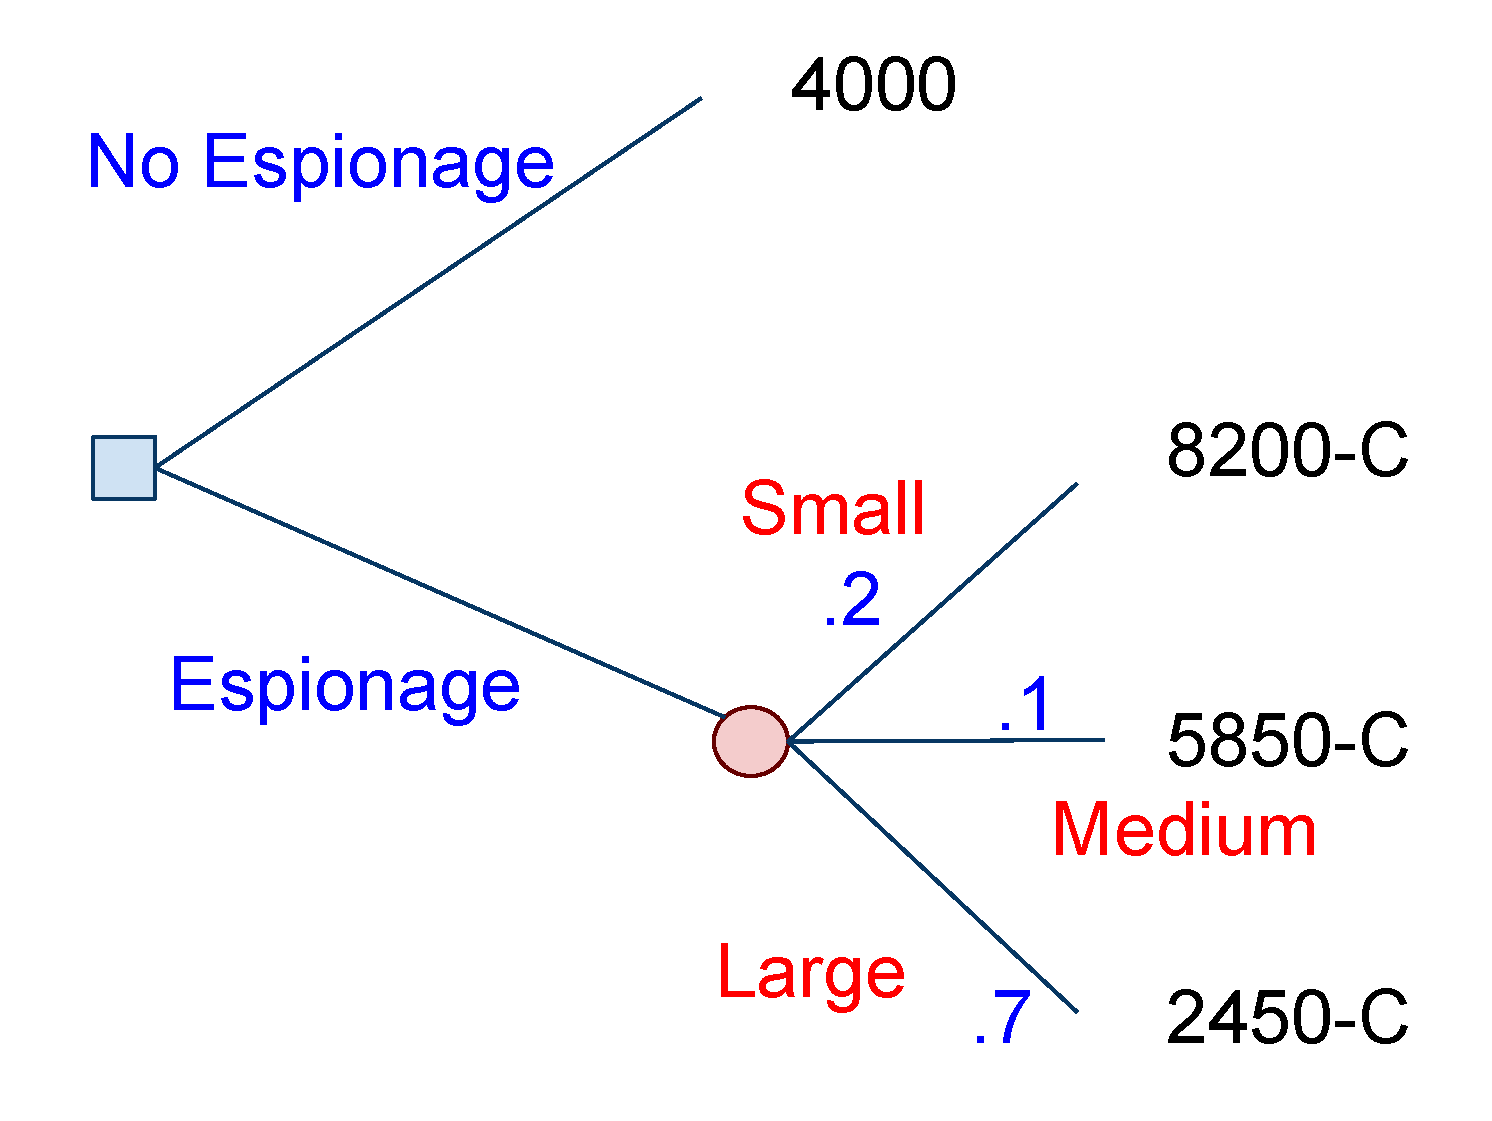
\includegraphics[width=7cm]{Espionage_Diagram.pdf}
\end{center}


Thus the expected return for ``Espionage'' is $3940-C$ and so ``Espionage'' is never the correct decision (unless $C$ is negative).

\item A reduced version of the tree is shown:

\begin{center}
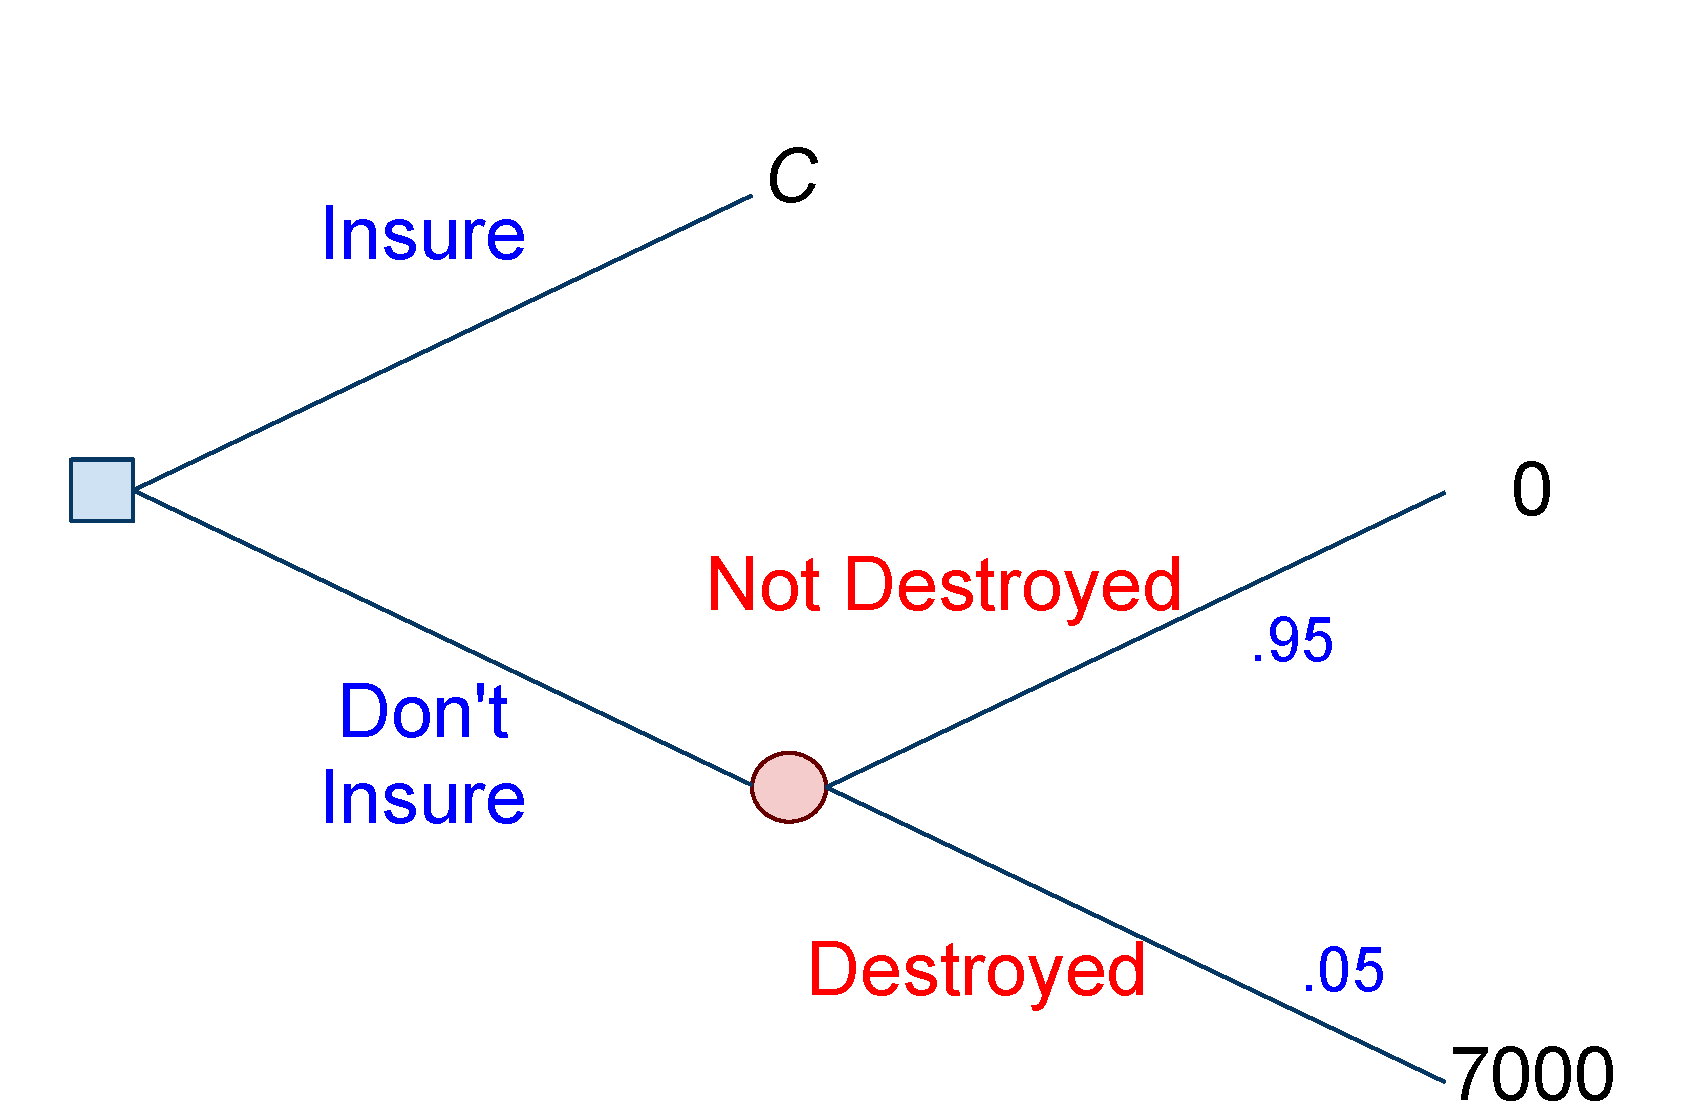
\includegraphics[width=7cm]{Insurance_Example.pdf}
\end{center}

It is worth (financially!) getting insurance if $\sqrt{C+1000}\leq .95\sqrt{1000}+.05\sqrt{8000}$ which reduces to $C\leq191.201$.

\item A risk averse strategy implies that the required decision is to ``not flip''. Thus we need $4000^{1\over n}\geq{1\over2}10000^{1\over n}$. Solving this inequality gives:
    $$\begin{array}{@{}r@{\;}c@{\;}l@{}}
    {1\over n}\ln4000&\geq& {1\over n}\ln10000-\ln2\\[2mm]
    {1\over n}\ln{5\over2}&\leq& \ln2\\[2mm]
    n&\geq& {\ln{5\over2}\over\ln{2}}\approx1.32
    \end{array}
    $$
    However since $n\in\mathbb{Z}$, this gives $n\geq2$. From the above equation we see that the important factor is the ratio of the two payoffs. Importantly this mean that \textbf{millions} or \textbf{thousands} will give the same result.

\item
Let:

\begin{itemize}
\item $D$ denote the event ``purchase from dealer''.
\item $P$ denote the event ``purchase privately''.
\item $AA$ denote the event ``get the AA to check''.
\item $NoAA$ denote the event ``not using the AA''.
\item $F$ denote the event ``the second hand car is faulty''.
\item $NoF$ denote the event ``the second hand car is not faulty''.
\item $AAfF$ denote the event ``the AA finds a fault''.
\item $AAdfF$ denote the event ``the AA does not find a fault''.
\end{itemize}

From the question we have:
$$\begin{array}{@{}r@{\;}c@{\;}l@{}}
P(F)=P(NoF)&=&.5\\[2mm]
P(AAfF\;|\;F)&=&.8\\[2mm]
P(AAfF\;|\;NoF)&=&0\end{array}$$

thus:

$$
\begin{array}{@{}r@{\;}c@{\;}l@{}}
P(AAfF)&=&P(AAfF\;|\;F)P(F)+P(AAfF\;|\;NoF)P(NoF)=.8\times.5+0={2\over5}\\[2mm]
P(AAdfF)&=&1-P(AAfF)={3\over5}\\[2mm]
P(F\;|\;AAfF)&=&{P(F)P(AAfF\;|\:F)\over P(AAfF)}=1\\[2mm]
P(noF\;|\;AAfF)&=&0\\[2mm]
P(F\;|\;AAdfF)&=&{P(F)P(AAdfF\;|\:F)\over P(AAdfF)}={1\over6}\\[2mm]
P(noF\;|\;AAdfF)&=&{5\over6}
\end{array}$$


\begin{center}
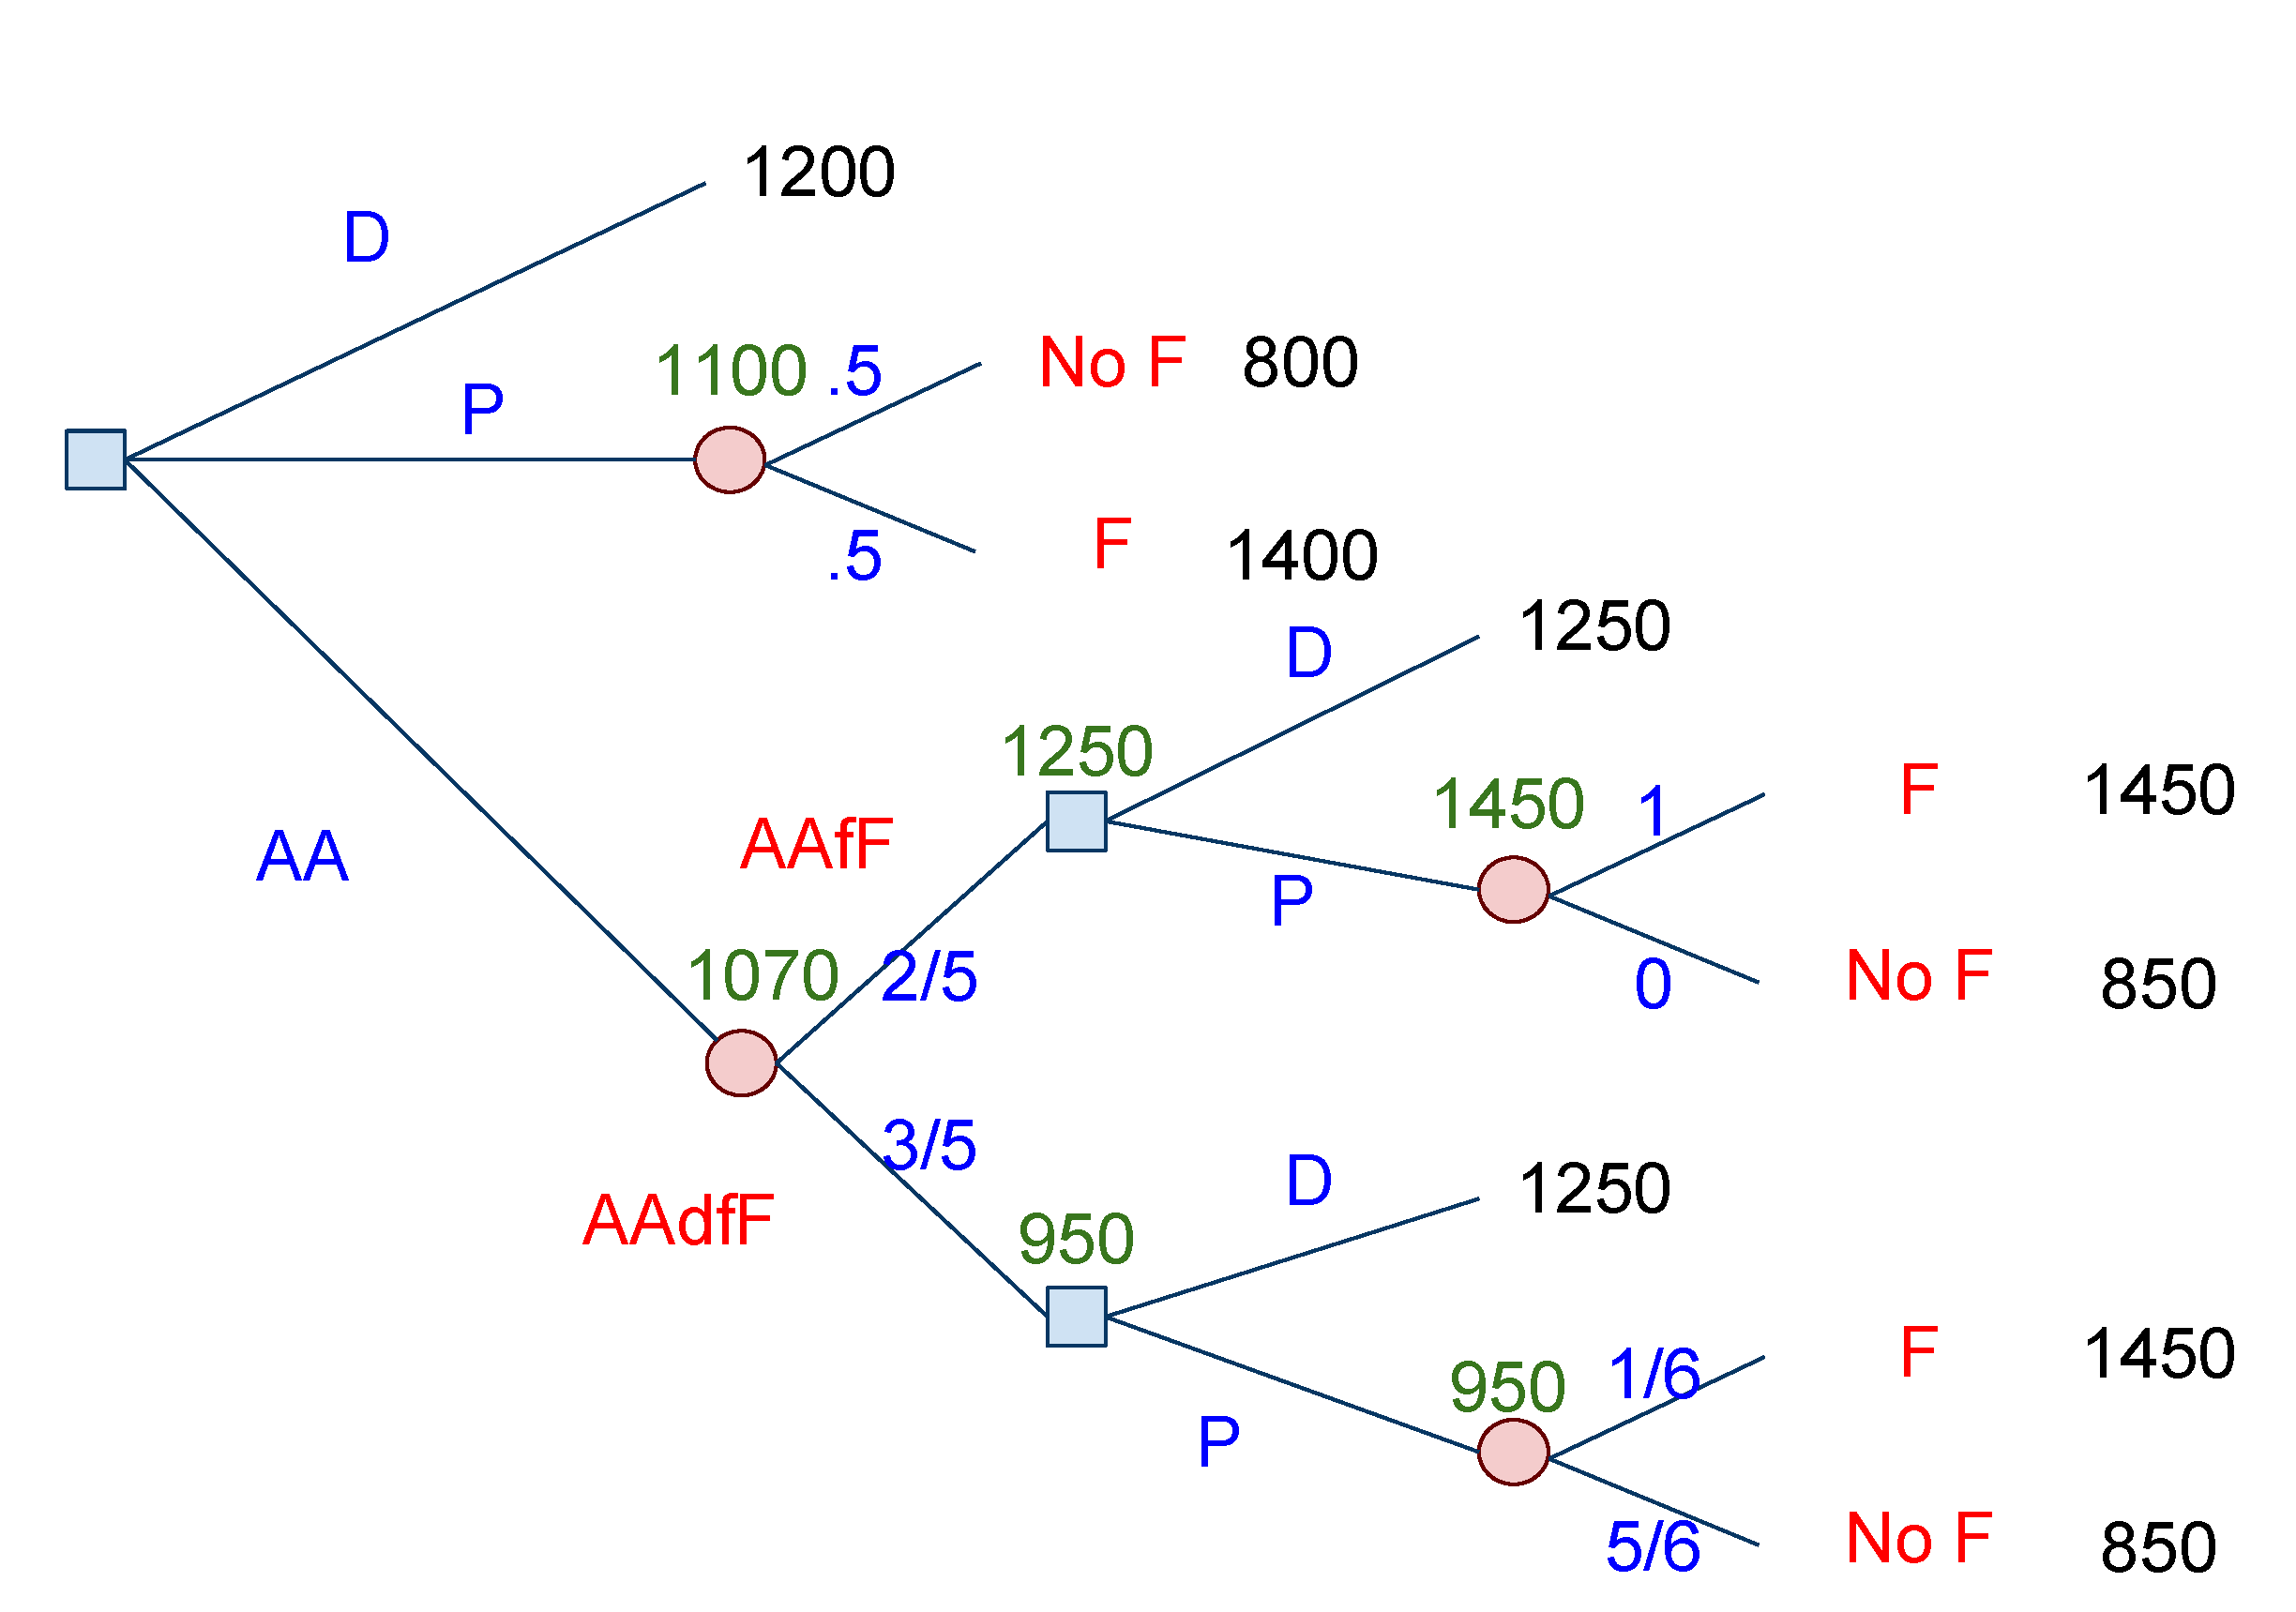
\includegraphics[width=12cm]{Car_Example.pdf}
\end{center}
thus the best financial option is to seek the AAs advice.
\end{enumerate}


\end{document}
